
\documentclass[parskip]{scrartcl}
\usepackage[margin=15mm]{geometry}
\usepackage{tikz}
\usetikzlibrary{shapes,backgrounds}

\newcommand{\tstar}[5]{% inner radius, outer radius, tips, rot angle, options
\pgfmathsetmacro{\starangle}{360/#3}
\draw[#5] (#4:#1)
\foreach \x in {1,...,#3}
{ -- (#4+\x*\starangle-\starangle/2:#2) -- (#4+\x*\starangle:#1)
}
-- cycle;
}

\newcommand{\ngram}[4]{% outer radius, tips, rot angle, options
\pgfmathsetmacro{\starangle}{360/#2}
\pgfmathsetmacro{\innerradius}{#1*sin(90-\starangle)/sin(90+\starangle/2)}
\tstar{\innerradius}{#1}{#2}{#3}{#4}
}

\begin{document}


\begin{tikzpicture}
 \tstar{2}{4}{7}{10}{thick,fill=blue}
\end{tikzpicture}
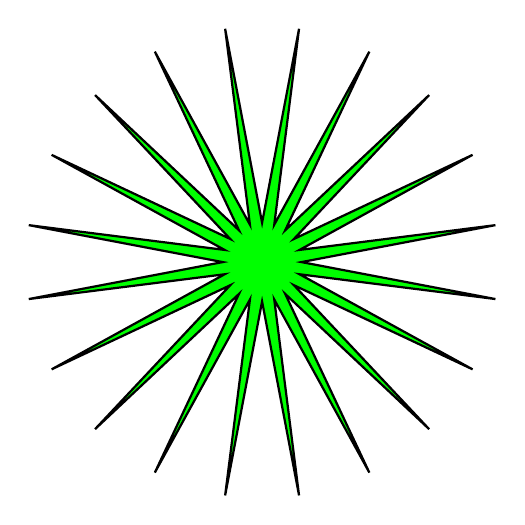
\begin{tikzpicture}
 \tstar{0.5}{3}{20}{0}{thick,fill=green}
\end{tikzpicture}


\begin{tikzpicture}
 \ngram{4}{5}{45}{thick,fill=red}
\end{tikzpicture}

\begin{tikzpicture}
 \ngram{4}{7}{0}{thick,fill=yellow}
\end{tikzpicture}

\end{document}